\chapter[Metodologia]{Metodologia}


\section{Métodos Ágeis}
\label{sec:Métodos Ágeis}

Neste capítulo são apresentados conceitos sobre as metodologias de
desenvolvimento ágil, bem como algumas filosofias abordadas por ela.

As metodologias de desenvolvimento ágeis têm origem com a publicação
do Manifesto Ágil \cite{manifestoAgil} que agrega princípios e valores, listados a

\begin{itemize}
  \item Indivíduos e interações mais que processos e ferramentas;
    \item Software em funcionamento mais que documentação abrangente;
    \item Colaboração com o cliente mais que negociação de contratos;
    \item Responder a mudanças mais que seguir um plano.
\end{itemize}

Para BECK et al \cite{manifestoAgil}, por mais que exista valor nos itens à direita da
frase, os itens a esquerda são mais valorizados nessa metodologia.
Segundo \cite{pressman}, o surgimento das metodologias ágeis foi uma
estratégia de sanar os empecilhos vigentes da engenharia de software tradicional.


A metodologia apresenta inúmeros benefícios, porém, não pode ser aplicada em
qualquer projeto de desenvolvimento, produtos, pessoas e situações. Para cada
ambiente existe uma metodologia que atenda melhor as necessidades específicas
Nessa linha de pensamento, \cite{pressman} diz que os métodos ágeis
são muito convenientes para projetos que estão em constante mudança e que as
necessidades são alteradas em um período de tempo curto.

Isso é permitido
devido à política de entrega de uma pequena parte do software pronta para o
cliente, com ciclos curtos, chamados de iterações.
Como consequência das filosofias ágeis, SOARES (2004) observou que
há uma grande preocupação com a otimização do tempo, ao ter um esforço
menor com documentação desnecessária para alcançar o produto final e mais
devoção para produção.

De acordo com \cite{soares}, o desenvolvimento ágil também é
conhecido por ser adaptativo ao invés de preditivo. Nos processos utilizando
odelo cascata, o planejamento e escopo são inteiramente definidos no começo
do projeto. Esse planejamento tem um custo elevado, além de ser extremamente
complexo, pois o escopo não pode ser alterado durante o desenvolvimento do
software. Esse fato pode trazer a insatisfação do cliente, pois as suas
necessidades podem mudar com o decorrer do tempo. Se houver algum erro no
planejamento, ele será encontrado apenas na entrega final para o cliente.

Como já dito por \cite{pressman}, o modelo ágil soluciona esses
problemas com entregas de produtos funcionais para o cliente em ciclos curtos. A
cada ciclo, o cliente pode avaliar se o que foi desenvolvido está dentro das suas
necessidades e quais as necessidades futuras são esperadas para a próxima
entrega. Esta política diminui o risco da perda de trabalho por um planejamento
errado, por um requisito mal interpretado ou mal implementado e por retrabalho
ao implementar novamente o mesmo requisito do cliente.

As metodologias ágeis vem se tornando constante em projetos de
desenvolvimento de software. Segundo \cite{dubakov}, no
próprio ano de 2008, 70\% das organizações estavam utilizando métodos ágeis
para a produção de software.

\section{Metodologia Utilizada}
\label{sec:Metodologia Utilizada}

Para o nosso processo de desenvolvimento, iremos utilizar o Scrum e como referência para
este, o Guia do Scrum \cite{guiaScrum}.

Nosso projeto adotará várias práticas do Scrum, dentre elas a divisão interna dos times de
desenvolimento. Iremos dividir em três papeis chamados de Time Scrum: Product Owner, Time de Desenvolvimento
 e Scrum Master, bem como definidos a seguir:

 \subsection{Product Owner}
 \label{subs:Product Owner}
O Product Owner, ou dono do produto, é o responsável por maximizar o valor do produto e do
trabalho do Time de Desenvolvimento. Como isso é feito pode variar amplamente através das
organizações, Times Scrum e indivíduos.

O Product Owner é a única pessoa responsável por gerenciar o Backlog do Produto. O
gerenciamento do Backlog do Produto inclui:

\begin{itemize}
\item  Expressar claramente os itens do Backlog do Produto;
\item Ordenar os itens do Backlog do Produto para alcançar melhor as metas e missões;
\item  Garantir o valor do trabalho realizado pelo Time de Desenvolvimento;
\item  Garantir que o Backlog do Produto seja visível, transparente, claro para todos, e mostrar o que o Time Scrum vai trabalhar a seguir; e,
\item Garantir que o Time de Desenvolvimento entenda os itens do Backlog do Produto no nívelnecessário.
\end{itemize}

O Product Owner pode fazer o trabalho acima, ou delegar para o Time de Desenvolvimento
fazê-lo. No entanto, o Product Owner continua sendo o responsável pelos trabalhos.

O Product Owner é uma pessoa e não um comitê. O Product Owner pode representar o desejo
de um comitê no Backlog do Produto, mas aqueles que quiserem uma alteração nas
prioridades dos itens de Backlog devem convencer o Product Owner.

Para que o Product Owner tenha sucesso, toda a organização deve respeitar as suas decisões.
As decisões do Product Owner são visíveis no conteúdo e na priorização do Backlog do
Produto. Ninguém tem permissão para falar com o Time de Desenvolvimento sobre diferentes
configurações de prioridade, e o Time de Desenvolvimento não tem permissão para agir sobre
o que outras pessoas disserem.

\subsection{Time de Desenvolvimento}
\label{sub:Time de Desenvolvimento}

O Time de Desenvolvimento consiste de profissionais que realizam o trabalho de entregar uma
versão usável que potencialmente incrementa o produto “Pronto” ao final de cada Sprint.
Somente integrantes do Time de Desenvolvimento criam incrementos.

Os Times de Desenvolvimento são estruturados e autorizados pela organização para organizar
e gerenciar seu próprio trabalho. A sinergia resultante aperfeiçoa a eficiência e a eficácia do
Time de Desenvolvimento como um todo. Os Times de Desenvolvimento tem as seguintes
características:

\begin{itemize}

  \item Eles são auto-organizados. Ninguém (nem mesmo o Scrum Master) diz ao Time de
  Desenvolvimento como transformar o Backlog do Produto em incrementos de
  funcionalidades potencialmente utilizáveis;
\item Times de Desenvolvimento são multifuncionais, possuindo todas as habilidades necessárias,
  enquanto equipe, para criar o incremento do Produto.
\item O Scrum não reconhece títulos para os integrantes do Time de Desenvolvimento que não
  seja o Desenvolvedor, independentemente do trabalho que está sendo realizado pela
  pessoa; Não há exceções para esta regra.
\item  Individualmente os integrantes do Time de Desenvolvimento podem ter habilidades
  especializadas e área de especialização, mas a responsabilidade pertence ao Time de
  Desenvolvimento como um todo; e,
\item Times de Desenvolvimento não contém sub-times dedicados a domínios específicos de
  conhecimento, tais como teste ou análise de negócios
\end{itemize}


\subsection{Scrum Master}
\label{sub:Scrum Master}

O Scrum Master é responsável por garantir que o Scrum seja entendido e aplicado. O Scrum
Master faz isso para garantir que o Time Scrum adere à teoria, práticas e regras do Scrum. O
Scrum Master é um servo-líder para o Time Scrum.

O Scrum Master ajuda aqueles que estão fora do Time Scrum a entender quais as suas
interações com o Time Scrum são úteis e quais não são. O Scrum Master ajuda todos a
mudarem estas interações para maximizar o valor criado pelo Time Scrum.

\subsubsection{O Scrum Master trabalhando para o Product Owner}
\label{subs:O Scrum Master trabalhando para o Product Owner}

O Scrum Master serve o Product Owner de várias maneiras, incluindo:

\begin{itemize}

\item  Encontrando técnicas para o gerenciamento efetivo do Backlog do Produto;
\item Claramente comunicar a visão, objetivo e itens do Backlog do Produto para o Time de
  Desenvolvimento;
\item Ensinar a Time Scrum a criar itens de Backlog do Produto de forma clara e concisa;
\item  Compreender a longo-prazo o planejamento do Produto no ambiente empírico;
\item  Compreender e praticar a agilidade; e,
\item  Facilitar os eventos Scrum conforme exigidos ou necessários.
\end{itemize}



\subsubsection{O Scrum Master trabalhando para o Time de Desenvolvimento}
\label{subs:O Scrum Master trabalhando para o Time de Desenvolvimento}

O Scrum Master serve o Time de Desenvolvimento de várias maneiras, incluindo:

\begin{itemize}
\item  Treinar o Time de Desenvolvimento em autogerenciamento e interdisciplinaridade;
\item  Ensinar e liderar o Time de Desenvolvimento na criação de produtos de alto valor;
\item  Remover impedimentos para o progresso do Time de Desenvolvimento;
\item  Facilitar os eventos Scrum conforme exigidos ou necessários; e,
\item  Treinar o Time de Desenvolvimento em ambientes organizacionais nos quais o Scrum não é
totalmente adotado e compreendido.
\end{itemize}


\subsubsection{O Scrum Master trabalhando para a Organização}
\label{subs:O Scrum Master trabalhando para a Organização}

O Scrum Master serve a Organização de várias maneiras, incluindo:
\begin{itemize}
\item  Liderando e treinando a organização na adoção do Scrum;
\item  Planejando implementações Scrum dentro da organização;
\item  Ajudando funcionários e partes interessadas a compreender e tornar aplicável o Scrum e o
desenvolvimento de produto empírico;
\item  Causando mudanças que aumentam a produtividade do Time Scrum; e,
\item  Trabalhando com outros Scrum Masters para aumentar a eficácia da aplicação do Scrum
nas organizações.
\end{itemize}

\subsection{Eventos Scrum}
\label{sub:Eventos Scrum}

O Guia do Scrum \cite{guiaScrum} traz também diretrizes sobre os eventos que acontecem dentro
do processo. Dentre elas temos a Sprint, Reunião Diária, Reunião de Retrospectiva e Revisão da Sprint,
assim como são listadas abaixo de acordo com o guia \cite{guiaScrum}

\subsubsection{Sprint}
\label{subs:Sprint}
O coração do Scrum é a Sprint, um time-boxed de um mês ou menos, durante o qual um
“Pronto”, versão incremental potencialmente utilizável do produto, é criado. Sprints tem
durações coerentes em todo o esforço de desenvolvimento. Uma nova Sprint inicia
imediatamente após a conclusão da Sprint anterior

\subsubsection{Reunião Diária}
\label{subs:Reunião Diária}

A Reunião Diária do Scrum é um evento time-boxed de 15 minutos, para que o Time de
Desenvolvimento possa sincronizar as atividades e criar um plano para as próximas 24 horas.
Esta reunião é feita para inspecionar o trabalho desde a última Reunião Diária, e prever o
trabalho que deverá ser feito antes da próxima Reunião Diária.

\subsubsection{Revisão da Sprint}
\label{subs:Revisão da Sprint}
A Revisão da Sprint é executada no final da Sprint para inspecionar o incremento e adaptar o
Backlog do Produto se necessário. Durante a reunião de Revisão da Sprint o Time Scrum e as
partes interessadas colaboram sobre o que foi feito na Sprint. Com base nisso e em qualquer
mudança no Backlog do Produto durante a Sprint, os participantes colaboram nas próximas
coisas que podem ser feitas para otimizar valor. Esta é uma reunião informal, não uma reunião
de status, e a apresentação do incremento destina-se a motivar e obter comentários e
promover a colaboração.

\subsubsection{Retrospectiva da Sprint}
\label{subs:Retrospectiva da Sprint}

A Retrospectiva da Sprint é uma oportunidade para o Time Scrum inspecionar a si próprio e
criar um plano para melhorias a serem aplicadas na próxima Sprint.

A Retrospectiva da Sprint ocorre depois da Revisão da Sprint e antes da reunião de
planejamento da próxima Sprint. Esta é uma reunião time-boxed de três horas para uma Sprint
de um mês. Para Sprint menores, este evento é usualmente menor. O Scrum Master garante
que o evento ocorra e que os participantes entendam seu propósito. O Scrum Master ensina
todos a mantê-lo dentro do time-box. O Scrum Master participa da reunião como um membro
auxiliar do time devido a sua responsabilidade pelo processo Scrum.

\section{Aplicação do Scrm no CIAC}
O projeto de desenvolvimento do CIAC irá utilizar a metologia Scrum.
Serão adotadas três releases, cada uma com seu timebox dentro do período dos pontos
de controle: PCx, onde x = \{1, 2, 3\}, estabelecidos pelos professores da disciplina no plano de ensino.

Dentro de cada release, foram definidas várias sprints, cada uma com o timebox
de uma semana. O marco para término da sprint é segunda feira, onde as atividades
serão desenvolvidas até o dia anterior. Há um encontro presencial em todos os dias
de término da sprint, onde, são executadas as reuniões de Revisão da Sprint,
Retrospectiva da Sprint e Planejamento da Sprint contendo todas as equipes
do projeto.

O projeto é composto por cinco times Scrum, cada um com seu Scrum master.
O conjunto de Scrum masters é dirigido pelos dois Products Managers: Tainara e Renato.

As demais equipes estão organizadas como a figura a seguir:
\begin{figure}[h]
  \centering
  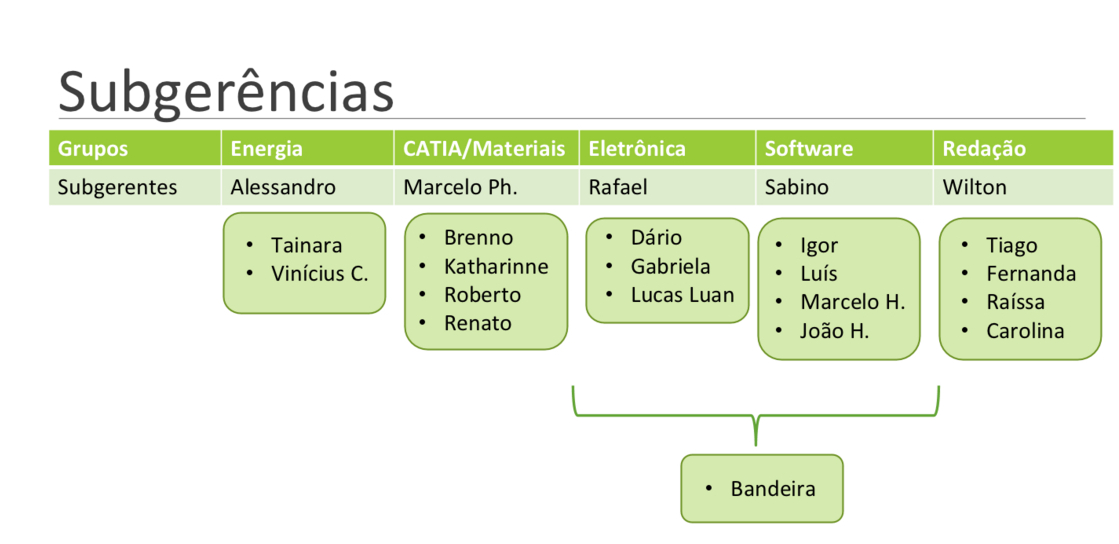
\includegraphics[width=400px, scale=1]{figuras/time}
  \caption{Divisão dos times}
\label{fig:time}
\end{figure}
Como pode ser visto na figura \ref{fig:time}, cada time irá tratar de um propósito no trabalho
ligado as cinco engenharias.
Cada um desses grupos tem atividades prórprias que remetem o seu escopo.

A partir da primeira release, surgiu o grupo de redação, responsável por escrever
o relatório e formatá-lo nos padrões exigidos. Além disso, existe um scrum master
responsável por gerencias os times de eletrônica e software. Essa decisão foi tomada,
pois, há muita interação entre as equipes, assim, este é responsável por fazer a ligação
de ambas as partes que devem estar em sincronia.

O backlog do produto é gerenciado pelos Products Managers e dividido aos Scrum Masters(Subgerente).
Cada time de desenvolvimento trabalha a partir de um Sprint Backlog destinado a cada
subgerente naquela semana de desenvolvimento e validado no dia da reunião de revisão
da sprint.

\section{Ferramentas de Comunicação e Desenvolvimento}
\subsection{Slack}
A plataforma de comunicação em grupo Slack foi adotada pelo grupo como meio de comunicação principal.
Sendo centralizada nela as principais informações e debates relevantes ao escopo do projeto.

\begin{figure}[h]
  \centering
  
\includegraphics[width=300px, scale=0.5]{figuras/slack}
  \caption{Plataforma de Comunicação Slack}
  \label{table:slack}
\end{figure}


\subsection{WhatsApp}
O WhatsApp foi escolhido como meio de comunicação secundário enquanto todos os integrantes do grupo
não migrassem para a plataforma principal. Lá se concentraram os esforços de contato inicial para reunir
todos os integrantes da equipe.

\begin{figure}[h]
  \centering
  
\includegraphics[width=300px, scale=0.5]{figuras/wpp}
  \caption{Plataforma de Comunicação WhatsApp}
  \label{table:wpp}
\end{figure}


\subsection{Trello}
O Trello foi escolhido como meio de gerenciamento de projetos, definindo grupos e
frentes de trabalho. Cada um com a sua devida atividade.

\begin{figure}[h]
  \centering
  
\includegraphics[width=300px, scale=0.5]{figuras/trello1}
  \caption{Plataforma de Gerência de Projetos}
  \label{table:trello1}
\end{figure}


\subsection{Google Drive}
O Google Drive foi escolhido como ferramenta para armazenamento dos arquivos e artefatos importantes para a
equipe. As entregas parciais de documentos e pesquisas dos integrantes foram todas centralizada nesta plataforma
para efeitos de backup de documentos.
\begin{figure}[h]
  \centering
  
\includegraphics[width=300px, scale=0.5]{figuras/google_drive-logo}
  \caption{Ferramenta de Armazenamento Google Drive}
  \label{table:google_drive-logo}
\end{figure}
\subsection{Latex}
O \LaTeX\ foi a ferramenta designada para a estruturação e escrita do relatório.
\begin{figure}[h]
  \centering
  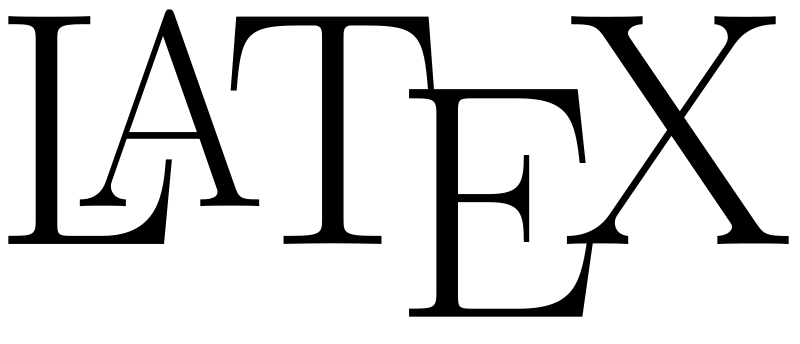
\includegraphics[width=200px, scale=0.5]{figuras/latex_logo}
  \caption{Ferramenta de Marcação de Texto LaTeX}
  \label{table:latex_logo}
\end{figure}
\subsection{Git}
Como ferramenta de versionamento utilizou-se o Git para gerenciar as mudanças e atualizações do conteúdo do slide
por todos os membros da equipe. Essa ferramenta foi escolhida pelo grupo para evitar diferenças e centralização do
conteúdo do relatório. Pois o mesmo foi armazenado em um repositório online para acesso de todos os membros do projeto.
\begin{figure}[h]
  \centering
  
\includegraphics[width=200px, scale=0.5]{figuras/git}
  \caption{Ferramenta de Versionamento GitHub}
  \label{table:git}
\end{figure}
\subsection{Editores de Texto}
\label{sub:Editores de Texto}
Para editar o textos compilados em LaTeX foram utilizados dois editores de texto diferentes:
\begin{itemize}
  \item Sublime text Editor
  \item Atom text Editor
\end{itemize}

\begin{figure}[h]
  \centering
  
\includegraphics[width=200px, scale=0.5]{figuras/sublime}
  \caption{Editor de Texto Sublime}
  \label{table:sublime}
\end{figure}
\begin{figure}[h]
  \centering
  
\includegraphics[width=200px, scale=0.5]{figuras/atom}
  \caption{Editor de Texto Atom}
  \label{table:atom}
\end{figure}
